\graphicspath{{images/}}

\section{\thesection~Introduction}
\label{sec:introduction}

% Expand motivation, describe QFA, discuss alternative approaches.

% Dummy \citet{Lawless2010} citations \citep{Heydari2016} \citep{Addinall2008}.

% The bacteria \textit{Eschericia Coli} and yeast \textit{Saccharomyces
%   cerevisae} are unicellular organisms studied as a model prokaryote
% and eukaryote respectively. They grow in colonies, where cells may (be
% clones originating from a single cell or) belong to different genetic
% strains originating from different individual cells. In favourable
% conditions, growth is exponential and this makes growth rate a major
% component of fitness; faster growing strains quickly come to dominate
% the population. Growth rate is measurable and is often used to
% determine the fitness of microbial organisms. For unicellular
% organisms, growth rate is equal to cell cycle progression
% rate. Evolutionary pressure has led to rapidly dividing organisms with
% a compact genome of essential genes. These genes have been conserved
% in other species over billions of years of evolution. The eukaryote
% \textit{S. cerevisae}, is particularly useful for the study of other
% eukaryotes such as humans.


The bacteria \textit{Eschericia Coli} and yeast \textit{Saccharomyces
  cerevisae} are unicellular organisms studied as a model prokaryote
and eukaryote respectively. Bacteria and yeast grow in colonies, where
cells may (be clones originating from a single cell or) belong to
different genetic strains originating from different individual
cells. In favourable conditions, growth is exponential and this makes
growth rate a major component of fitness; faster growing strains
quickly come to dominate the population. At a certain point growth
becomes limited and a stationary phase is reached. For unicellular
organisms, growth rate is equal to cell cycle progression rate and all
of the genetic information must be copied before each division. As a
result, evolutionary pressure has led to rapidly dividing organisms
with compact genomes of essential genes. These genes have been
conserved in other species over billions of years of evolution, which
is, in part, what makes \textit{E. Coli} and \textit{S.  cerevisae}
useful as model species. The eukaryote \textit{S. cerevisae}, is
particularly useful for the study of other eukaryotes such as humans.

The growth rate of microbial organisms is measurable and is often used
to determine fitness. In experiments, cell cultures are commonly grown
in two types of medium: on the surface of a nutrient rich solid agar
and in a liquid mixture containing nutrients. (REMOVE: In spot tests
(phenotypic array), cultures are pinned or inoculated on the surface
of a solid agar containing nutrients. In liquid culture assays,
cultures are mixed in a liquid medium containing nutrients.) In both
cases cultures are incubated and growth is observed. Identical strains
can grow differently between the two mediums and disagreement in
fitness estimates is currently an issue \citet{Baryshnikova2010} (I
couldn't find a paper specifically talking about this issue but they
have a correlation plot Fig2a where correlations are worse with a
liquid culture study by Jasnos and Korona; in fact the Baryshnikova
paper Fig3c seems to say that they had strong correlation in their
``high-resolution liquid growth profiling study''). I do not focus on
this issue and exclusively study fitness screens using solid agar.

% Where do cells grow surfaces films.

%%% Genetic interaction, SGA and QFA %%%

% Synthetic Genetic Array (SGA) and Quantitative Fitness Analysis (QFA)
% are high-throughput methods for obtaining quantitative fitness
% estimates of microbial cultures grown on solid agar
% \citep{Baryshnikova2010sga,Banks2012}.

% Fitness estimates can be used to infer genetic interaction or drug
% response and high-throughput methods allow this to be done on a
% genome-wide scale (see e.g. \citet{Costanzo2010}). In a typical
% genetic interaction study, a strain is made with a mutation in a query
% gene. Double mutants are created by introducing a second deletion in
% this strain. Typically one query gene is used per plate with
% replicates of many different deletions. By comparing the growth of
% double mutants with a control containing a neutral deletion, genetic
% interactions can be inferred. If a strain is fitter than the control
% then the deletion is said to suppress the defect of the query gene. If
% a strain is fitter than the control then the deletion is said to
% enhance the defect of the query gene. Either scenario suggests that
% the two genes interact and have a related function. Typically one
% query gene is used per plate and many replicates of each deletion are
% contained on each plate. Many plates can be analysed in
% high-throughput to explore whole genomes.


Fitness estimates can be used to infer genetic interaction or drug
response and high-throughput methods allow this to be conducted on a
genome-wide scale (see e.g. \citet{Costanzo2010,Andrew2013}). In a
typical genetic interaction screen a strain is made with a mutation in
a query gene. Double mutants are created by introducing a second
deletion in this strain. By comparing the growth of double mutants
with a control containing a neutral deletion, genetic interactions can
be inferred. If a strain is fitter than the control then the deletion
is said to suppress the defect of the query gene. If a strain is less
fit than the control then the deletion is said to enhance the defect
of the query gene. Either scenario suggests that the two genes
interact and have a related function. Due to redundancy, single
deletions are often non-lethal. (Remove: Knock downs and conditional
mutations can also be used.) This has allowed \citet{Costanzo2010} to
explore genetic interactions for \(\sim\)75\% of the
\textit{S. cerevisae} genome.


Synthetic Genetic Array (SGA) and Quantitative Fitness Analysis (QFA)
are high-throughput methods for obtaining quantitative fitness
estimates of microbial cultures grown on solid agar
\citep{Baryshnikova2010sga,Banks2012}. Typically one query gene and
replicates of several deletions are pinned or inoculated in a
rectangular array on a solid agar plate. Many plates with different
query genes and deletions are grown in high-throughput to explore
whole genomes. I study data from QFA which refers to quantitative
estimation of fitness by measurement and fitting of growth curves. In
a typical QFA procedure liquid cultures are incolulated onto solid
agar (containing nutrients (already mentioned above)) in a 16x24
rectangular array of 384 spots. Inoculum density can be varied to
capture more or less of the growth curve and the most dilute cultures
are inoculated with \(\sim\)100 starting cells
\citep{Addinall2011}. Plates are grown in incubation and removed to be
photographed at timepoints throughout growth. Photographs are of whole
plates and growth typically covers several days to capture both the
exponential and stationary growth phases. Colonyzer
\citep{Lawless2010} processes optical density measurements in
photographs to produce a timecourse of cell density estimates for each
culture. In pasts analysis, the logistic growth model was
independently fit to the timecourse of each culture and fitness
estimates were defined in terms of parameters of this model: the
growth constant \(r\) and carrying capacity \(K\). In contrast, SGA
typically uses a larger array of 1536 pinned cultures and a single
endpoint assay of culture area to quantify growth. The the
differential form and solution of the logistic model
\citep{Verhulst1845} (probably don't need this reference) are given in
Equations~\ref{eq:logistic_model}, where \(C\) represents cell density
and \(C_{t_{0}}\) is cell density at time zero.
% Logistic model equations
\begin{subequations}
  \label{eq:logistic_model}
  \begin{align}
    &\dot{C} = rC\left(1 - \frac{C}{K}\right)\\
    &C(t) = \frac{KC_{t_{0}}e^{rt}}{K + C_{t_{0}}(e^{rt}-1)}
  \end{align}
\end{subequations}
%
The logistic model is a simple mechanistic model describing
self-limiting growth and has a sigmoidal solution. Growth begins
exponentially with rate \(rC\) and curtails as the population size
increases and cells begin to compete for space and nutrients (remove:
or interact in some other way). Cell density reaches a final carrying
capacity \(K\) at the stationary phase. In QFA, nutrients must diffuse
through agar to reach cells growing on the surface. It is plausible
that the carrying capacity \(K\) represents the point at which
nutrients either run out or growth becomes limited by the diffusion of
nutrients and is approximately stationary. Fitting the logistic model
to QFA data requires plate level or culture level parameters for
\(C_{t_{0}}\) and culture level parameters for \(r\) and \(K\) making
769 or 1152 parameters per 384 culture plate.

//Could remove and just discus MDR when I get to the results//
The growth constant \(r\) could be used as a fitness measure. However,
\citet{Addinall2011} define a more complicated fitness measure as the
product of Maximum Doubling Rate (MDR) and Maximum Doubling Potential
(MDP) which they calculate from logistic model parameters. MDR measures
the doubling rate at the beginning of the exponential growth phase,
when growth is fastest, and MDP is the number of divisions which a
culture undergoes from inoculation to the stationary phase.
%
\begin{subequations}
  \label{eq:MDR_MDP}
    \begin{align}
      MDR &= \frac{r}{log\left(\frac{2(K-C_0)}{K-2C_0}\right)}\\
      MDP &= \frac{log\left(\frac{K}{C_0}\right)}{log(2)}
    \end{align}
\end{subequations}
%
To improve the quality of fits, QFA now uses the generalised logistic
model which requires an extra shape parameter for each
culture. Standard and generalised logistic model \(r\) are not
equivalent so comparison relies on MDR and MDP as fitness
measures. The analysis of QFA data using both models is available
through the QFA R package \citep{qfa2016}.  //Could remove and just
discus MDR when I get to the results//


//Could remove//\citet{Addinall2011} used QFA and
\textit{S. cerevisae} to screen for genes involved in telomere
stability which is related to ageing and cancer and has implications
for human health and disease. Hits from this study have been
successfully followed to discover new biology
\citep{Holstein20141259}. (To be honest I have no idea about the
significance of what they found in this paper. We had a more general
focus. If I have room I should probably try and sell the potential
benefits and past successes of QFA a bit more to expand the
motivation. Obviously I will mention the Addinall paper when I
describe p15 in the methods.)  //Could remove//
% Example use of QFA by Addinall \citep{Addinall2011} telomeres.
% And follow up Holstein and Clark \citep{Holstein20141259}


Since QFA aims to determine differences in the fitness of microbial
strains from measurements of differences in growth, fast and slow
growing cultures are often grown
side-by-side. Figure~\ref{fig:p15_section} shows a section of a QFA
plate from a study by \citeauthor*{Addinall2011} where this is the
case. (Cultures were inoculated with approximately equal cell density
but have grown at different rates to visibly different sizes after
\(\sim\)2.5 days.) Despite starting with the same amount of nutrients
and growing at different rates there is a characteristic timescale for
the cessation of growth. This suggests a global growth limiting effect
which I believe to be caused by an interaction between cultures. I
test the hypothesise that the interaction is a competition effect due
to the diffusion of nutrients along gradients formed between fast and
slow growing neighbours. This has implications for growth estimates;
competition will cause growth to appear faster or slower for each
neighbour than would be observed if they were grew independently. The
experiment shown in Figure~\ref{fig:stripes_images} provides further
support for a nutrient competition effect. The same cultures were
grown in alternate columns on two separate plates but with cultures
added or removed from the neighbouring columns inbetween. Cultures in
Figure~\ref{fig:stripes_images}a), where neighbours were removed, grew
faster and larger (how much? I can look at the data myself) than the
same cultures in Figure~\ref{fig:stripes_images}b), where neighbours
were added. This suggests that an interaction between neighbours is
present and may be affecting fitness estimates. Current QFA analysis
using the logistic model assumes that cultures grow independently and
ignores possible competition effects between neighbours. The sigmoidal
curve of the logistic model poorly fits QFA data in many cases and
this may be due to competition effects. I aim to fit a network model
of nutrient dependent growth and diffusion to QFA data to try to
correct for competition and increase the accuracy and precision of
fitness estimates.

Could explain the difference in dilute and more concentrated
cultures. In the image captions or elsewhere?\\\\
Could also talk about quorum sensing and amonia when I get to
competition.

% First edit checkpoint 1

\begin{Figure}
  \centering
  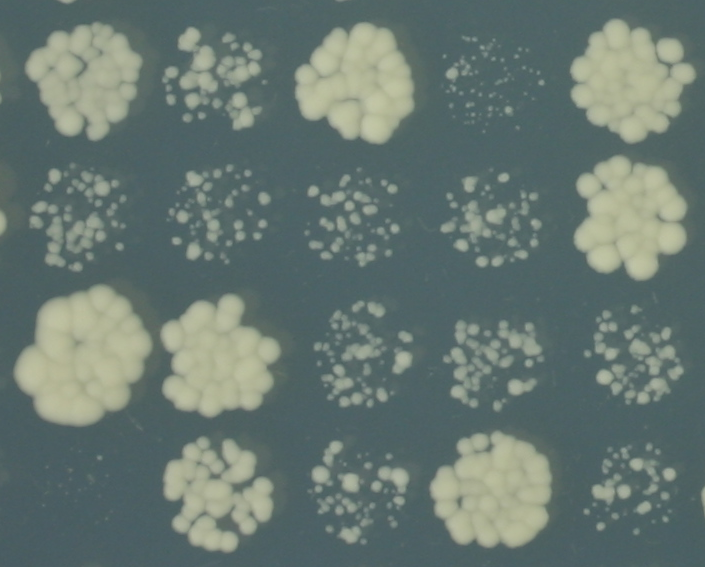
\includegraphics[width=\linewidth]{p15_section/p15_section}
  \captionof{figure}{\textbf{4x5 section of a QFA plate.} Taken from a
    16x24 format solid agar plate inoculated with dilute
    \textit{S. cerevisae} cultures.
  Image captured at \(\sim\)2.5d after inoculation and incubation at
  27\(^{\circ}C\).}
  \label{fig:p15_section}
\end{Figure}
\begin{Figure}
  \centering
  \includegraphics[width=\linewidth]{stripes/final/striped}
  \includegraphics[width=\linewidth]{stripes/final/filled}
  \captionof{figure}{\textbf{QFA experiment designed to examine
      competition.}  A) QFA plate inocluated with a more concentrated
    \textit{S. Cerevisae} inoculum (no cells inocluated on alternate
    columns). B) Same as in A, but with strains of similar growth rate
    inoculated in the positions missing in A.}
  \label{fig:stripes_images}
\end{Figure}

Competition effects could be dealt with experimentally by randomising
the location of cultures on repeated plates. This does not require
explicit knowledge or modelling of the source of competition but
reduces throughput, so, if possible, a modelling approach is
desirable. Poisoning of cultures by a signal molecule such as ethanol,
which \textit{S. cerevisae} produces in the metabolism of sugars by
fermentation, is another possible source of competition. QFA does not
measure nutrients or signal, so if more than one source of competition
exists, it becomes very difficult to fit a model and randomisation may
be the best approach. QFA data for edge cultures is noisy due to
reflections from plate edges. This is only partially corrected for by
Colonyzer \citep{Lawless2010} and as a result data for edge cultures
is usually discarded. \citet{Addinall2011} grow repeats of a neutral
deletion in edge locations, rather than leaving them empty, because of
concerns about competition. In an SGA study, \citet{Baryshnikova2010}
use statistical techniques to correct for competition between fast and
slow growing neighbours in end-point assays of culture area. I hope
that modelling competition for nutrients explicitly will better
correct for competition using fewer repeats. QFA uses more information
than SGA by fitting whole growth curves, rather than a single endpoint
assay, so a modelling approach promises to be more
powerful. Furthermore, modelling may identify and explain the source
of competition. Simulation of an accurate model will allow comparison
of experimental designs and exploration of ways to reduce competition
effects.

//Diffusion Equation: I am probably going to have to repeat this
when I get to the discussion so I could just leave until then.//
% Previous model of nutrient diffusion.
\citet{Reo2014} use a diffusion equation model to simulate nutrient
dependent growth of a single bacterial culture on a pertri dish in
two-dimensions. It would be too computationally intensive to fit a
similar model to a full QFA plate in three-dimensions, especially if
the model is to be used to process many plates from high-throughput
experiments. Therefore, a simpler model of nutrient diffusion is
required. //Diffusion Equation//


\textit{Lawless} (link blog) proposed a model of nutrient dependent
growth and competition (\ref{eq:reaction},\ref{eq:competition_model}),
hereinafter the competition model, using mass action kinetics and
network diffusion. A schematic of the model is drawn in
Figure~\ref{fig:comp_model_schematic}. He represents the nutrient
dependent division of cells with the reaction equation,
\begin{equation}
  \label{eq:reaction}
    C + N \xrightarrow[]{b} 2C,
\end{equation}
where \(C\) is a cell, \(N\) is the amount of nutrient required for
one cell division, and \(b\) is a rate constant for the reaction. (The
identity of the limiting nutrient \(N\) is unknown but possible
candidates are sugar and nitrogen.) He defines separate reactions
(\ref{eq:reaction}) with growth constant \(b_{i}\) for each culture,
indexed \(i\), on a plate and uses mass action kinetics to derive rate
equations for the amount of cells and nutrients associated with each
culture, \(C_{i}\) and \(N_{i}\). This gives the rate equation for
\(C_{i}\) (\ref{eq:competition_model}a) and the first term in the rate
equation for \(N_{i}\) (\ref{eq:competition_model}b).
\begin{subequations}
  \label{eq:competition_model}
  \begin{align}
    % \frac{dC_{i}}{dt}& = b_{i}N_{i}C_{i},\\
    % \frac{dN_{i}}{dt}& = - b_{i}N_{i}C_{i} - k_{n}\sum_{j \epsilon \delta_i}(N_{i} - N_{j}).
    \dot{C_{i}}& = b_{i}N_{i}C_{i},\\
    \dot{N_{i}}& = - b_{i}N_{i}C_{i} - k_{n}\sum_{j \epsilon \delta_i}(N_{i} - N_{j}).
  \end{align}
\end{subequations}
To arrive at the full competition model, he models the diffusion of
nutrients along gradients between a culture \(i\) and its closest
neighbours \(\delta_{i}\) by the second term in
(\ref{eq:competition_model}b), where \(k_{n}\) is a nutrient diffusion
constant. This can also be expressed as a series of reactions of the
form
\begin{subequations}
  \label{eq:diffusion_reaction}
  \begin{align}
  &N_{i} \xrightarrow[]{k_{n}} N_{j}\\
  &N_{j} \xrightarrow[]{k_{n}} N_{i},
  \end{align}
\end{subequations}
and modelled with mass action kinetics. Unlike the logistic
model~(\ref{eq:logistic_model}), the competition model has no
analytical solution, and must instead be solved numerically. If
\(k_{n}\) is set to zero, the competition model reduces to the mass
action equivalent of the logistic model, hereinafter the mass-action
logistic model, (and has the same sigmoidal solution). (In this limit,
parameters of the competition model can be converted in terms of
parameters the logistic model (see methods section)).
%%%% could go to methods %%%%
When the competition model is fit to QFA data, \(C_{i}\) is observed
and \(N_{i}\) is hidden. Inoculum density, \(C_{t_{0}}\), is often
below detectable levels. By assuming that incolulum density is the
same for all cultures and that nutrients are distributed evenly
throughout the agar at time zero, plate level initial values of cells
and nutrients, \(C_{t_{0}}\) and \(N_{t_{0}}\), can be used. \(k_{n}\)
is assumed to be constant across the plate but must be inferred. There
is a growth constant, \(b_{i}\), for each of 384 cultures on a typical
QFA plate making 387 parameters in total. The competition model shares
more information between cultures and has less than half the number of
parameters of either the standard or generalised logistic model
\citep{Banks2012,qfa2016}. (If I remove the section on MDR and the
generalised logistic model above I will need to add a line of
explanation here.)
%%%%%%%%%%%%%%%%%%%%%%%%%%%%%%%
\begin{Figure}
  \centering
  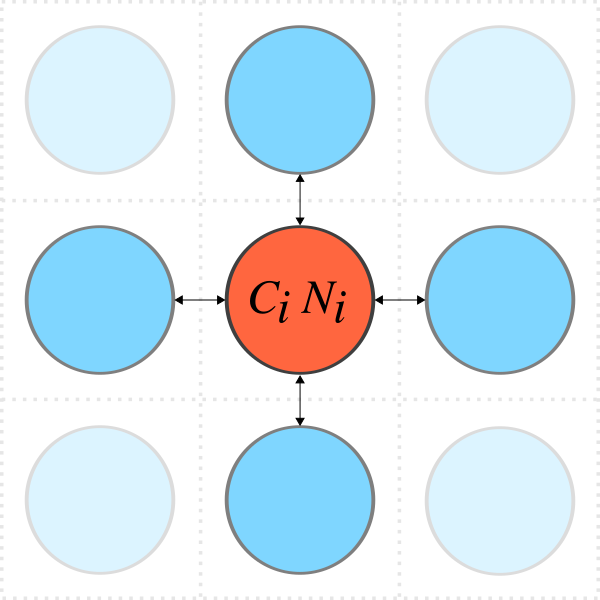
\includegraphics[width=\linewidth]{comp_model/comp_model_schematic}
  \captionof{figure}{\textbf{Schematic of the competition model.}
    Each circle represents a culture, indexed \(i\), growing in a
    rectangular array on the surface of a nutrient containing solid
    agar. Arrows represent a network of nutrient diffusion along
    gradients between cultures. \(C_{i}\) - amount of cells; \(N_{i}\)
    - amount of nutrients; \(k_{n}\) - plate level nutrient diffusion
    constant; darker blue circles \(\delta_{i}\) - closest neighbours
    of culture i.}
  \label{fig:comp_model_schematic}
\end{Figure}

In QFA, populations begin with \(\sim\)100 cells and quickly grow to
reach thousands of cells so a deterministic approximation appears
valid.  Mass action kinetics applies to reactions in a well stirred
mixture and is perhaps less valid for a culture growing on solid agar.
However, a mass action approximation has been successful in other
situations where this assumption is questionable: in the
Lotka-Volterra model of predator-prey dynamics \citep{Berryman1992}
and in signalling and reaction models inside cells
\citep{Aldridge2006,Chen2010}. The order of a reaction also affects
the rate equation and the identity and quantity of the nutrient
molecule in the (\ref{eq:reaction}) is unknown. Reaction
(\ref{eq:reaction}) also assumes that all nutrients are converted to
cells and includes no model of metabolism. I justify the use of the
competition model because in the independent limit it has the same
solution as the logistic model which has long been used to model
microbial growth. Studying the competition model may help us to
understand the nature of QFA experiments and, if some assumptions do
not hold, it could be used as a first step in developing a more
accurate model. Furthermore, collectively fitting the competition
model involves a the large number of parameters and data points and
will require many simulations to be run. This necessitates the use of
an approximate model for computational feasibility. This is especially
true if the model is to be used in the analysis of high-throughput
data. It is hoped that even an approximate model will be able to
measure more reliable growth parameters and better estimate
fitness. This will increase the power to infer genetic interaction and
drug response which could lead to further discoveries. (For an example
of a sucessful QFA study and follow up using the logistic model see
\citet{Addinall2011} and \citet{Holstein20141259}).

% Comment on all nutrients go to cells can wait until methods
% % Fractal kinetics can wait until the discussion.
% fractal kinetics if nutrient diffusion is limited inside cultures, due
% to gel-like properties of the medium \citep{savageau1995,Kopelman1988}
% \citep{savageau1995,Kopelman1988}

%%% Local Variables:
%%% mode: latex
%%% TeX-master: "report"
%%% End:
